\chapter{Introduction}
\label{chapter1}
\thispagestyle{plain}
GN Techonomy S.r.l. is a consulting company that, since 1995, offers technological and innovative enterprise solutions. GN techonomy is active in Information technology sector providing ERP (Enterprise resource planning) solutions as well as variety of customized software for its clients. The company’s mission statement is to develop a lasting competitive advantage for its customers. I chose this organization because I find their mission to be important and relevant to my career goals.
My role at GN  Techonomy is JAVA solution architect. This report aims to summarise a project which was developed for a customer of GN Techonomy during a six months period of time.

\section{Context}\label{sec:context}
Platforms operate in two-or multi-sided markets with distinct groups of end users. \cite{article_two_sided_platform} Their value lies in creating an interdependence between the different types of users in a way that facilitates transactions, thus improving the welfare of both. \cite{Lamadrid_2015}
Platforms operate online and offline, common offline examples are newspapers and shopping malls,while online ones include search engines and social networks. \cite{Rochet2005TheRC} Recent technological developments–notably computer software, the internet and smart phones have considerably expanded the scope for platforms to lower transaction costs. \cite{Munger2015}

According to a study performed by JPMorgan Chase Institute \cite{jpmorgan_2016} , there is a dramatic growth in number of individuals who are earning income from online platforms, such as Uber\footnote{Uber Technologies, Inc., commonly known as Uber, is an American multinational ride-hailing company offering services that include peer-to-peer ridesharing, ride service hailing, food delivery, and a micromobility system with electric bikes and scooters}, TaskRabiit\footnote{TaskRabbit is an American online and mobile marketplace that matches freelance labor with local demand, allowing consumers to find immediate help with everyday tasks, including cleaning, moving, delivery and handyman work}, or Airbnb\footnote{Airbnb, Inc. is an American online marketplace company based in San Francisco, California, United States. Airbnb offer arrangement for lodging, primarily homestays, or tourism experiences}.
In addition JPMorgan\&Chase researchers, also make a distinction between "labour" and "capital platforms", which they define as fallowing:
\textit{Labour platforms} such as Uber or TaskRabbit, often referred to as "Gig Economy" connect customers with freelancers or contingent workers who perform discrete tasks or projects,
\textit{Capital platforms} such as Ebay\footnote{eBay Inc. is an American multinational e-commerce corporation based in San Jose, California, that facilitates consumer-to-consumer and business-to-consumer sales through its website} or Airbnb connect customers with individuals who rent assets or sell goods peer to peer \cite{jpmorgan_2016}.

The result of their research indicates between October 2012 and September 2015, monthly participation in the Online Platform Economy grew 10-fold, from 0.1\% to 1.0\% (figure\ref{fig:participation_1}). In addition over this three-year period, the cumulative participation grew from 0.1\% of adults to 4.7\%, a 47-fold growth (figure\ref{fig:participation_2}). 


Global trends indicate that the number of people across the world using the internet has grown to 4.54 billion, an increase of 7 percent (298 million new users) from January 2019 to January 2020. Globally, more than 5.19 billion people now use mobile phones, with user numbers up by 124 million (2.4 percent) over the past year \footnote{https://datareportal.com/reports/digital-2020-global-digital-overview}. In addition, according to a statistics Portal 2017 survey, 88\% of Americans and 78\%  of French book their hotel using Internet \footnote{https://www.statista.com/statistics/666643/preference-of-online-or-offline-hotel-booking-us/}. 

The result of aforementioned study helps us classify our digital platform.
An online booking digital platform belongs to the category of \textit{Capital platforms}. In addition as the study suggests, it is evident that the number of adults participating in digital online platforms economy is increasing rapidly year by year. Considering the fact that the number of people across the world using the internet has increased by 7 percent (298 million new users) from Jan 2019 to January 2020 \footnote{https://datareportal.com/reports/digital-2020-global-digital-overview} we can confidently assume, existence of a tremendous potential for gaining profit from online platforms by means of taking advantage of the growing user base in order to monetize the platform for interested investors. In this report we will discuss the structure of such platforms in form of an online property booking system from a software engineering perspective.   

\begin{figure} 
\centering
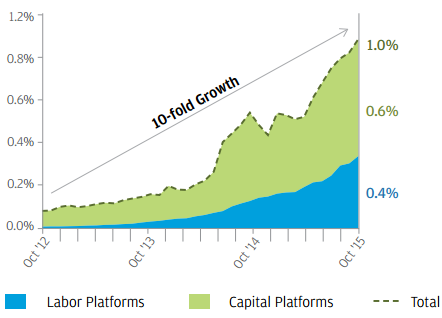
\includegraphics[width=8cm]{pictures/adults_1.png}
\caption{Year by year participation percentage}
Graph illustrates percentage of adults participating in the
Online Platform Economy in each month. Image courtesy JPMorgan Chase Institute\cite{jpmorgan_2016}.
\label{fig:participation_1}
\\
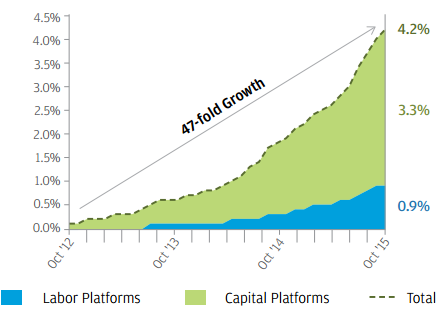
\includegraphics[width=8cm]{pictures/adults_2.png}
\caption{Year by year cumulative percentage} 
Graph illustrates cumulative percentage of adults who have ever
participated in the Online Platform Economy. Image courtesy JPMorgan Chase Institute\cite{jpmorgan_2016}
\label{fig:participation_2}
\end{figure} 

%Digital platform is defined as a common place which provider of a good/service is connected to the end consumer through the internet in order to facilitate the connection between two parties.


\section{Problem Statement}\label{sec:problem_statement}
Online booking platforms such as AirBnB offer arrangement for a short period hospitality, primarily connecting hosts (renters) and guests (typically tourists, students, etc.). One observation is that, the services provided by AirBnB or similar websites is not by design a "premium experience", there are cases of high profile, VIP guests which need to rent a property for example a villa, a house or a mansion in its entirety for possibly an extended period of time, in some cases even months.

This opens up opportunity for another digital platform which can connect the high end, luxury seeking guests with property owners which do not intend to enlist their properties on low end platforms such as AirBnB. Providing premium user experience is the main differentiating factor which needs to be embedded in every aspect of our digital platform. In chapter \ref{chapter3} we will discuss some guidelines on how to craft a better user experience.

First part of designing any piece of software project is the identification of already existing business processes among different actors, e.g. agencies enlisting properties, Realtor, VIP guest, etc. For this part interviewing the investors of the platform and identifying their requirements and expectations is necessary. 

The result of the interview between the project investor and software developer is as follows: 
A booking platform in essence should be capable of managing interactions between host(s) and guest(s). 
The host should be able to enlist his/her property on the platform specifying a period of availability and  a set of criteria for the guests including number of guests and the price for the property. Alternatively the guest should be able to filter listed properties on the platform based on his/her preferences which includes price,location, desired period, etc. and obviously book the chosen property.
Finally there is also an authority figure to manage conflicts between hosts and guests, this is defined as the platform administrator which in this project is defined as the platform manager.

After the identifying the scope and requirements of the project, we need to assess them in order to find out possible candidate technologies and methodologies, in order to design the software architecture solution which can firstly address the requirements, secondly speed up the business processes and finally increase productivity for the software customer as well as end users.  





%In this report we try to analyze the requirements proposed by the customer and design a software system which satisfies those requirements. We introduce suitable technologies for the implementation of the software system and discuss how they interact among each other.



%There are several approaches for identifying software requirements. The approach we use here agile user stories.
%A user story is an informal, natural language description of one or more features of a software system. User stories are often written from the perspective of an end user or user of a system.




%\subsection{Description of }
%lorem ipsum
\section{Proposed Solution}\label{sec:proposed_solution}
After analyzing the investors requirements, as well as identifying end user needs through analysis of similar software, we chose a candidate solution, a website which addresses needs of the high end property owners as well as guests looking for luxury/high valued properties for rent. The website platform is capable of making profit for the investors through monetizing transactions between guests and hosts.
Another proposed solution was development of a mobile application encapsulating the same functionalities as the website, however throughout interviews with investors we found that, they prefer development of a web application due to the existence of previously built assets and capabilities, however they are in favor of extending the platform to mobile devices in the future. 

%investors and end users are not interested simply due to the fact that this segment of customers go through extensive planning and research before making decisions and the website is better suited to address their needs. 
 

In a nutshell, our solution boils down to development of a fully functional responsive website \footnote{Responsive web design is an approach to web design that makes web pages render well on a variety of devices and window or screen sizes.}, hosted by one of the well known cloud providers, which is capable of managing booking, reservation, handling transactions, making invoices and finally build reports for future analysis. The emphasis on "UX Design" in order to provide premium experience for the users is considered as well.

%In this thesis we discuss design and implementation of a software project in form of a web application for managing interactions among different entities namely host,guest and platform administrator.
%The interactions between different types of users can analyzed and identified through requirement analysis phase.

%The main idea is to design a digital platform which is able to connect two or more entities and facilitate communication among those entities, providing them with tools necessary to conduct transactions which in turn make the platform profitable.
\section{Thesis Structure}\label{sec:thesis_structure}
We already provided some context and back ground info about digital platforms in general and booking digital platform specifically throughout this  chapter. %throughout the second chapter
In he second chapter we will focus on technologies used for the implementation of our digital platform as well as methodologies which were chosen by the software development team.
In the third chapter we will go through software engineering blue print of the project and discuss the software architectural design thoroughly.
Finally in the fourth chapter we will discuss the implementation experience and process of validation by the customer and end users. The conclusion and possibility for future improvement of the software is discussed in the last chapter.

%In this thesis we mainly discuss design and implementation of the booking platform software through a software engineering perspective and only discuss briefly the underlying technologies used to implement the software.

